\clearpage
\section{Visualizing Movement}\label{sec:visualizing-movement}

Because the focus of our research is on artists' lives, this led to interest in movement and change of places during their lifetime. The space-time
path we saw in the previous section shows this movement trajectory in the space-time cube. To gain more information and knowledge about how the
movement is represented in other data visualizations, we will explore various visualization techniques which capture this phenomenon. We can
visualize a change from one point to another by drawing a link between nodes that represent points. The type of link depends on the visualization,
but usually, it is some kind of line. One of the diagrams that represent movement is called a flow map. We already saw an example of a flow map by
Minard in \Cref{fig:figure2.2}, but the idea for this visualization comes from engineer Henry Drury Harness in 1837. One of his maps shown in
\Cref{fig:figure2.14} presents the flow of cargo traffic quantity in Ireland~\citep{irish1838atlas, robinson19551837}.
Generally, the width of the lines in these kinds of maps indicates the number of objects being transferred~\citep{phan2005flow}.

\begin{figure}[h]
    \begin{center}
        \includegraphics[width=\textwidth]{graphics/2-literature-review/14}
    \end{center}
    \caption{The flow of cargo traffic}
    \label{fig:figure2.14}
\end{figure}

\clearpage

Migrations of people can also be represented circularly. A popular visualization for this is a chord diagram where nodes are placed on
the outer part of the circle and connected among each other by arcs. The size of an arc, like the line in the flow map, is proportional to
the number of people or objects moving. Below we can see an example of a chord diagram taken from~\citep{baptista2018internal}. It shows the
migration flows in the Brazilian states between 2005 and 2010.

\begin{figure}[h]
    \begin{center}
        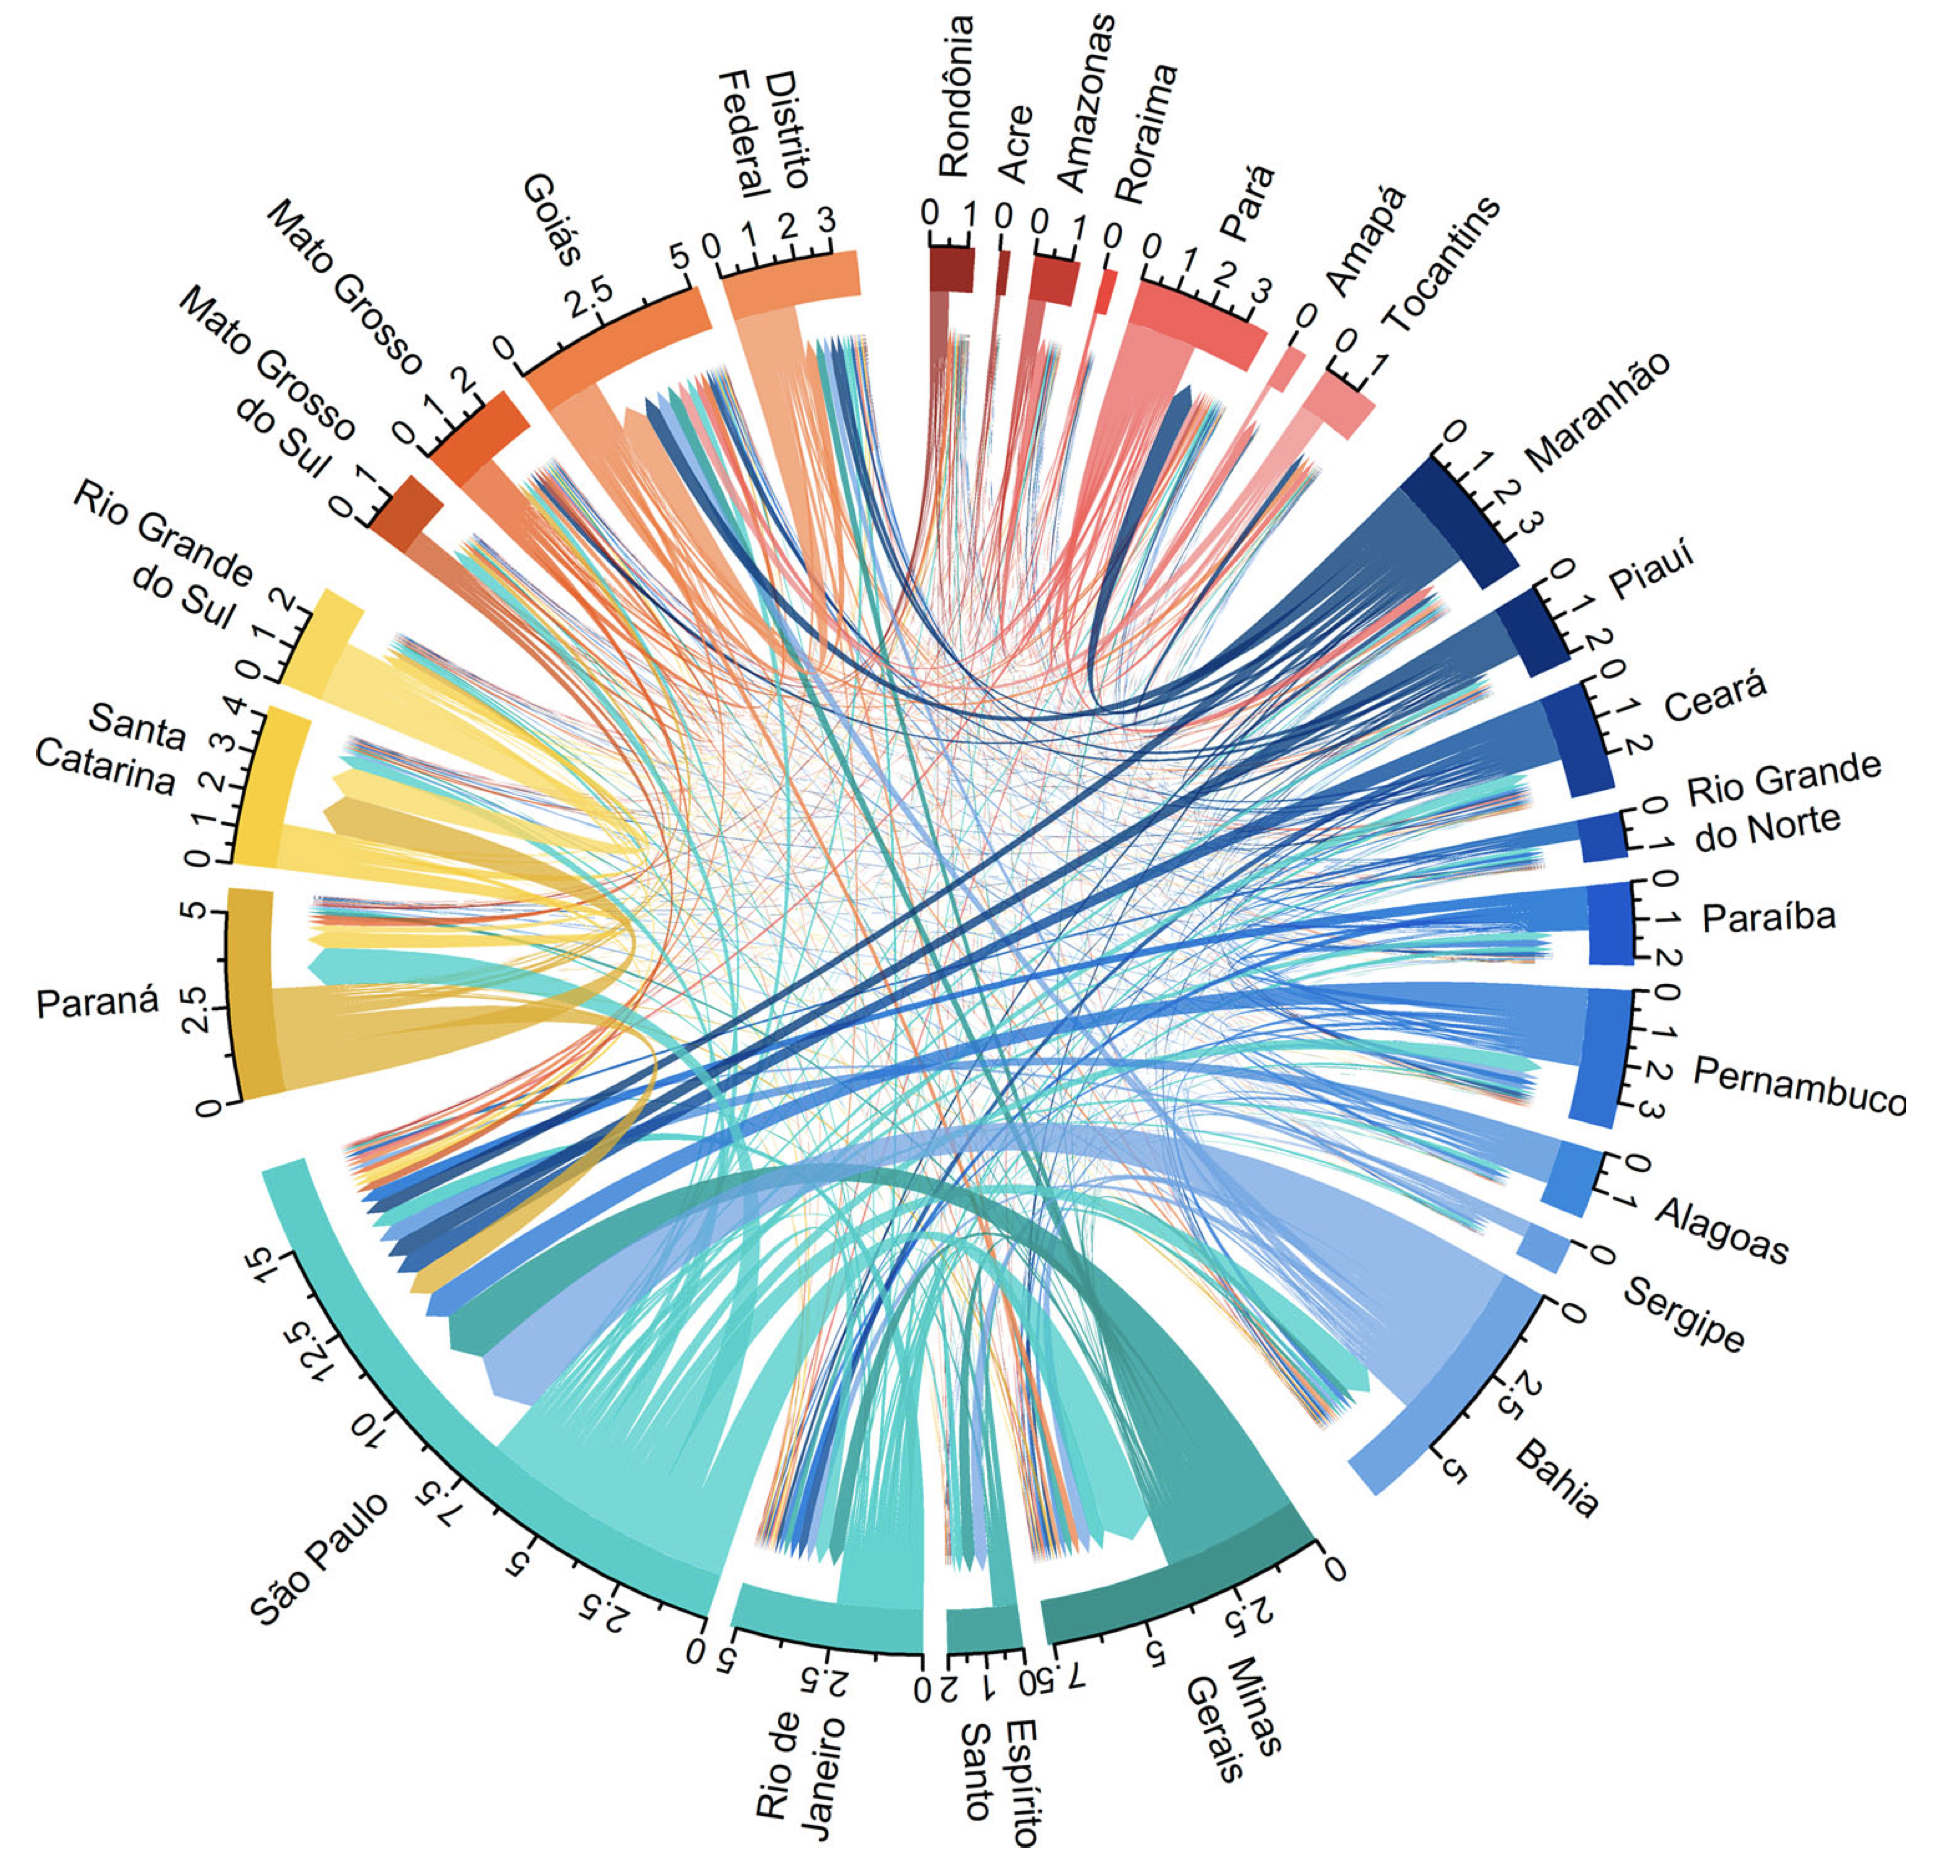
\includegraphics[width=0.7\textwidth]{graphics/2-literature-review/15}
    \end{center}
    \caption{A chord diagram of migration flow in Brazilian states (thousands)}
    \label{fig:figure2.15}
\end{figure}

Chord diagrams are often interactive because they allow a better visual aspect of the data. The static ones can seem tangled and hard to
understand if there are too many arcs. The interactive part usually allows the user to highlight only a selected arc, while others may change
the color to become less visible and neutral, and the selected one stands out for a better view.\footnote{You can see an example of an
interactive chord diagram on the website\\ \url{http://download.gsb.bund.de/BIB/global_flow/}}
Rees et al.~\citep{rees2020interaction} introduce more engaging interaction techniques for chord diagrams.

A very interesting data visualization of the migration of artists found in the Rijksmuseum database is the one by
Koeleman~\citep{koeleman2017visualizing}. In this interactive chart, it is possible to hover over the cities on the outer part of the circle
or a country in the inner part for the migrations related to it to lighten.\footnote{Chart can be found on the website
\url{http://visualizingvisions.com}} The red lines show the immigration patterns, while the blue ones show the emigration. We can see that most
of the artists are from the Netherlands (not surprising as the Rijksmuseum is in Amsterdam), but a more interesting discovery is that artists
from various nationalities moved to Italy, while the Italian ones only moved within the country.

\begin{figure}[h]
    \begin{center}
        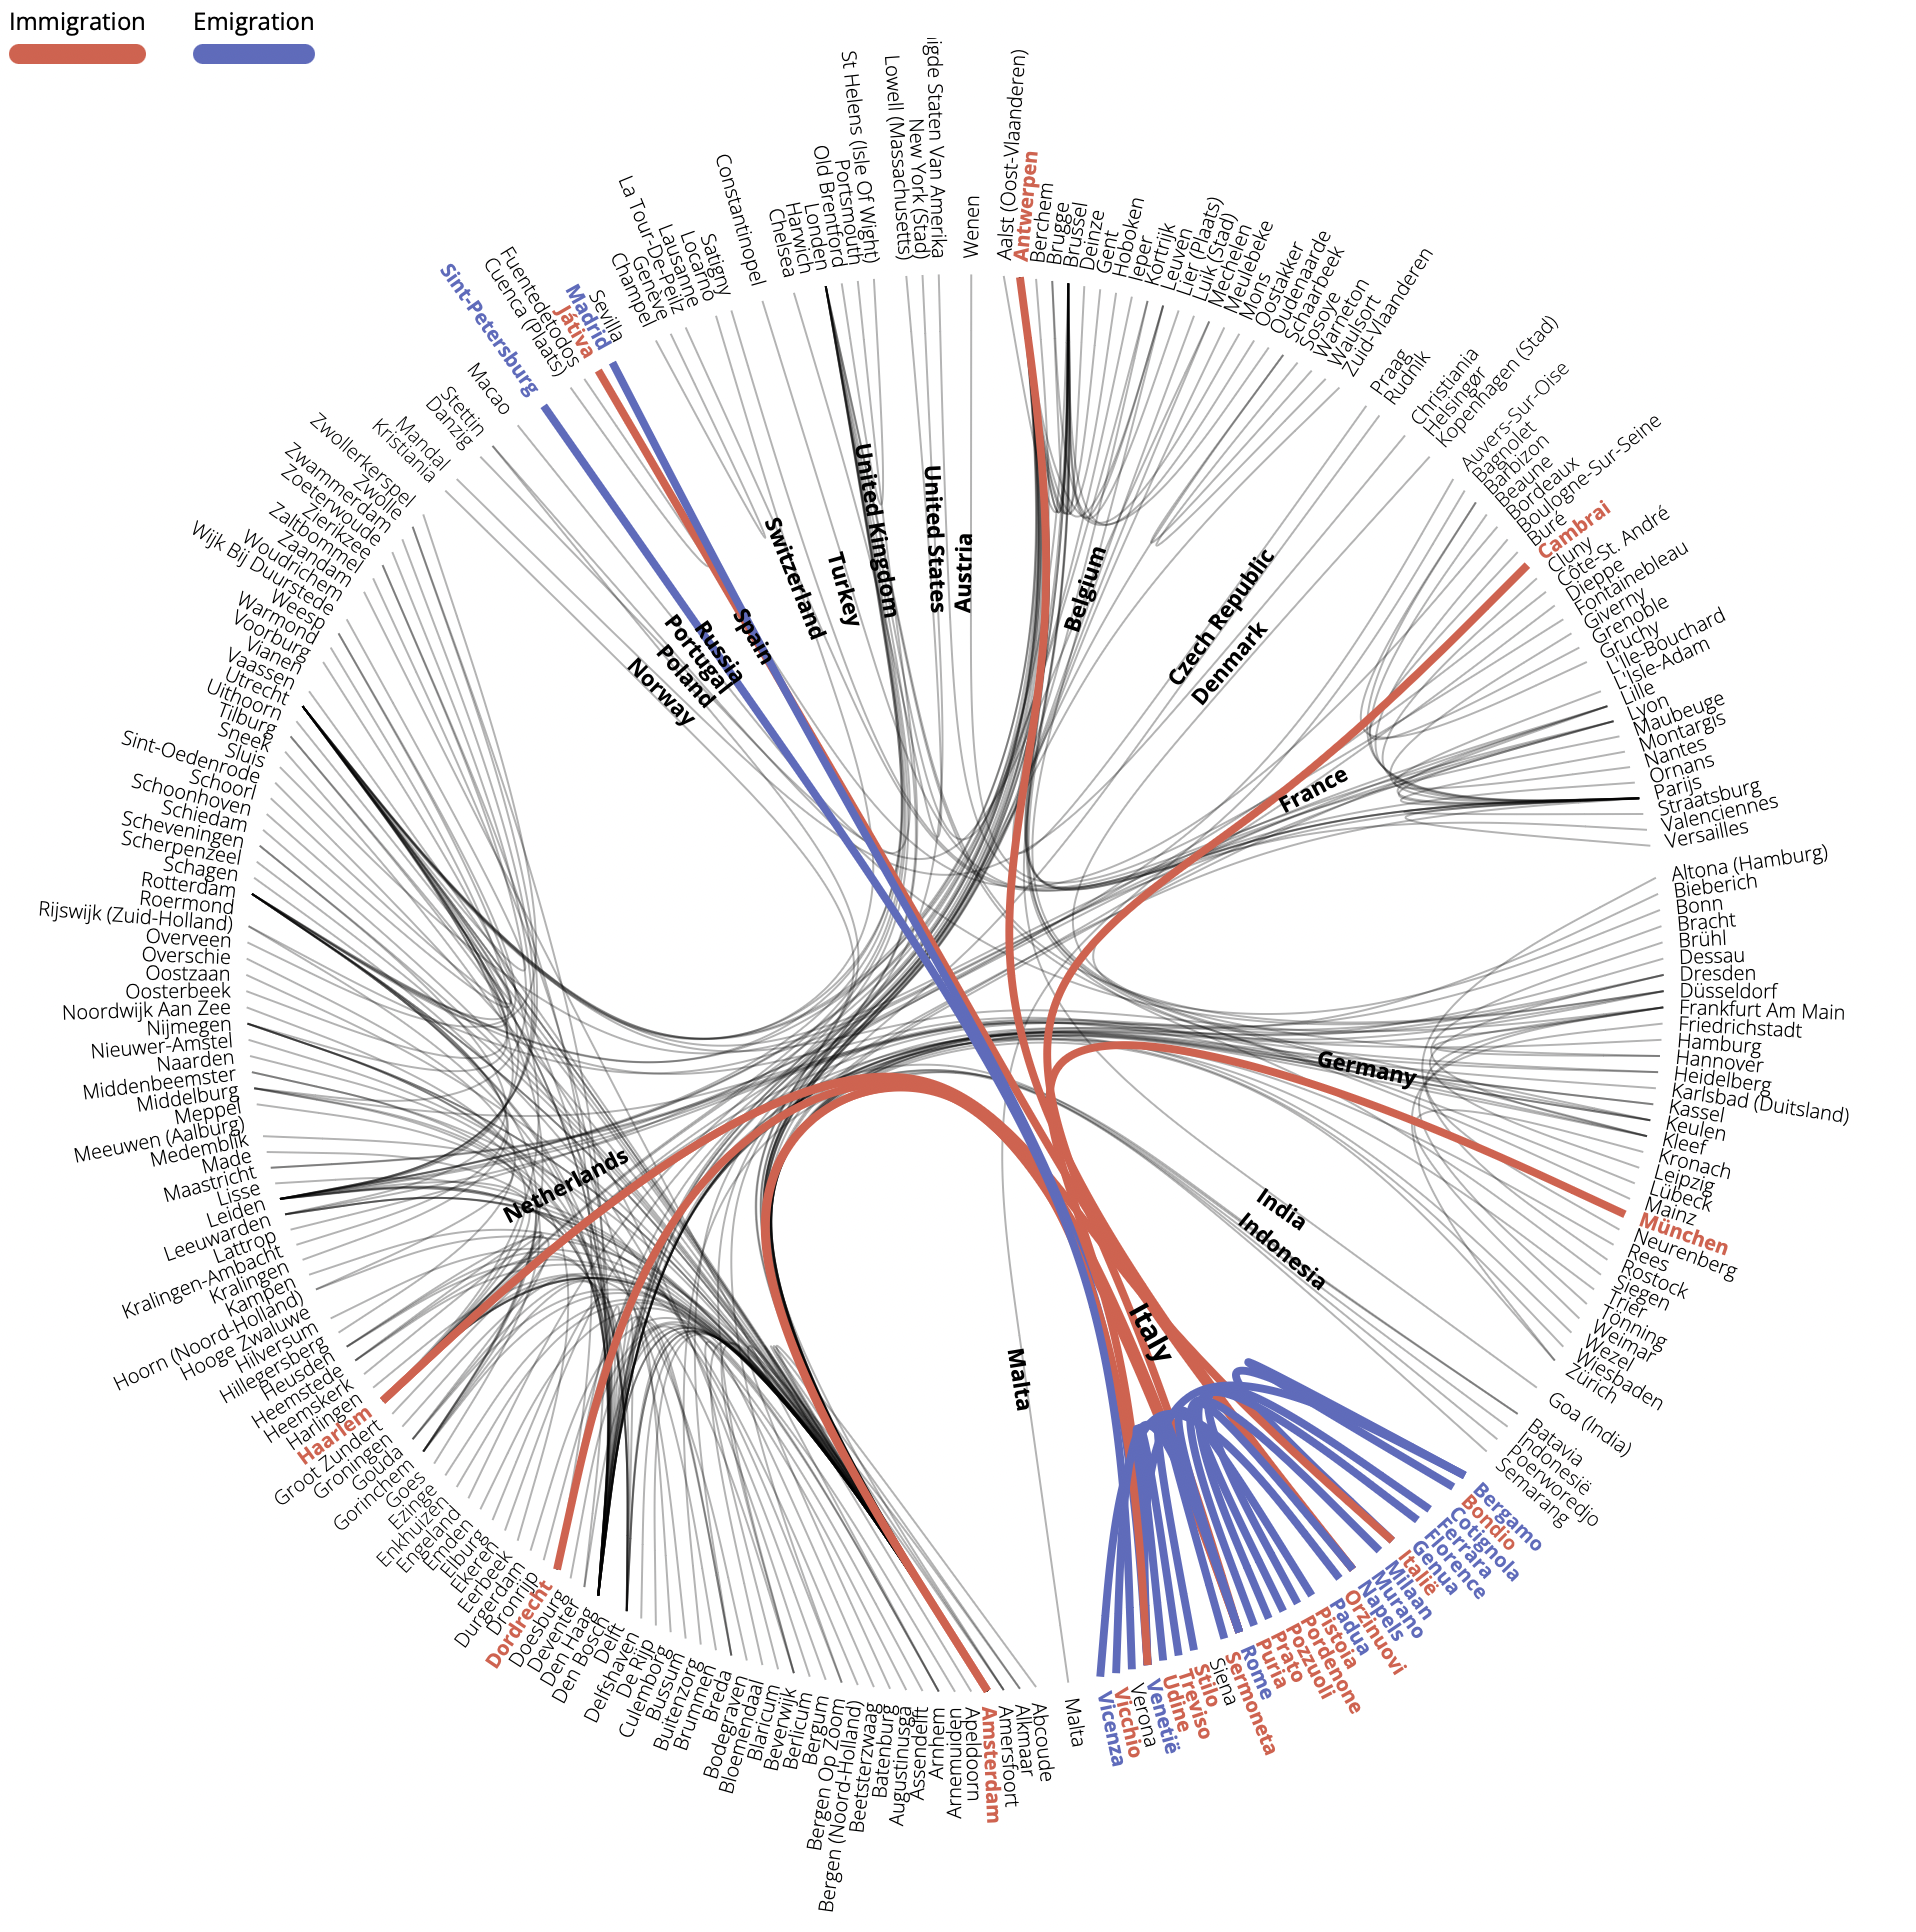
\includegraphics[width=0.9\textwidth]{graphics/2-literature-review/16}
    \end{center}
    \caption{Migration of artists found in Rijksmuseum database}
    \label{fig:figure2.16}
\end{figure}

These visualizations show that the representation of the movement of people usually includes a big amount of data. It enables
searching for a pattern and understanding what happened in general, not focusing much on a single person as an object of observation. Besides, they
do not offer a lot of details about locations and their spatial relationships. Because we are interested in the life of an artist as an individual,
these types of data visualizations are not suitable for the implementation part. Even though exploring relationships with other artists as well
gives us more data to work with, it would still be ineffective to use them because they are only concerned with the migration part. Nevertheless,
characteristics can still be taken from these charts and implemented in our work. For example, the property of a width of a line we saw in
\Cref{fig:figure2.14} can be used in our space-time cube to represent some aspect of an artist's life, such as the number of artworks they have
created during a certain period or any other.
